\item {\bf Linear Classifiers (logistic regression and GDA)}

In this problem, we cover two probabilistic linear classifiers we have covered in class so far. First, a discriminative linear classifier: logistic regression. Second, a generative linear classifier: Gaussian discriminant analysis (GDA). Both the algorithms find a linear decision boundary that separates the data into two classes, but make different assumptions. Our goal in this problem is to get a deeper understanding of the similarities and differences (and, strengths and weaknesses) of these two algorithms.

For this problem, we will consider two datasets, along with starter codes provided in the following files:
\begin{center}
\begin{itemize}
	\item \texttt{src-linear/ds1\_{train,valid}.csv}
	\item \texttt{src-linear/ds2\_{train,valid}.csv}
  	\item \texttt{src-linear/main.py}
	  \item \texttt{src-linear/submission/\_\_init\_\_.py}
	\item \texttt{src-linear/submission/logreg.py}
	\item \texttt{src-linear/submission/gda.py}
\end{itemize}
\end{center}
Each file contains $\nexp$ examples, one example $(x^{(i)}, y^{(i)})$ per row. In particular, the $i$-th row contains columns $x^{(i)}_0\in\Re$, $x^{(i)}_1\in\Re$, and $y^{(i)}\in\{0, 1\}$. In the subproblems that follow, we will investigate using logistic regression and Gaussian discriminant analysis (GDA) to perform binary classification on these two datasets.

\textbf{Code Deliverables}
\begin{itemize}
	\item \texttt{src-linear/submission/logreg.py}
	\item \texttt{src-linear/submission/gda.py}
	\item \texttt{src-linear/submission/\_\_init\_\_.py}
\end{itemize}

\begin{enumerate}
	\input{01-linearclass/01-logreg}
	\item \points{1b}
Follow the instructions in \texttt{src-linear/submission/logreg.py} to train a logistic regression classifier using Newton's Method. You will complete the |fit| and |predict| functions of the |LogisticRegression| class.

Starting with $\theta = \vec{0}$, run Newton's Method until the updates to $\theta$ are small: Specifically,  train until the first iteration $k$ such that $\vert\theta_{k} - \theta_{k-1}\vert_1 < \epsilon$, where $\epsilon = 1\times 10^{-5}$. Make sure to write your model's predicted probabilities on the validation set to the file specified in the code.

To verify a correct implementation, run the autograder test case |1b-4-basic| to create a plot of the \textbf{validation data} with $x_1$ on the horizontal axis and $x_2$ on the vertical axis. This plot uses a different symbol for examples $x^{(i)}$ with $y^{(i)} = 0$ than for those with $y^{(i)} = 1$. On the same figure, it will also plot the decision boundary found by logistic regression (i.e, line corresponding to $p(y\vert x) = 0.5$).

The output plot should look similar to the following (no plot submission is required): 

\begin{figure}[H]
	\centering
	\vspace{2mm}
	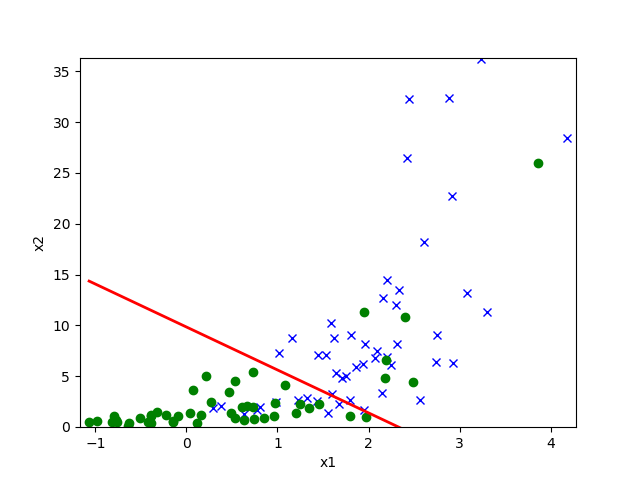
\includegraphics[width=0.65\linewidth]{01-linearclass/p01b_pred_1.png}
    \caption{Separating hyperplane for logistic regression on validation set of Dataset 1. Visual impaired students can access the corresponding desmos plot \href{https://www.desmos.com/calculator/vl5mh1k4q2}{here} (Note: This is for reference only.  You are not required to submit a plot.)}
\end{figure}

	\input{01-linearclass/03-gda}
	\input{01-linearclass/04-gda-ll}
	\item \points{1e}
In \texttt{src-linear/submission/gda.py}, fill in the code to calculate $\phi$, $\mu_{0}$, $\mu_{1}$, and $\Sigma$, use these parameters to derive $\theta$, and use the resulting GDA model to make predictions on the validation set. More specifically, you complete the |fit| and |predict| functions for the |GDA| class.

Make sure to write your model's predictions on the validation set to the file specified in the code. 

To verify a correct implementation, run the autograder test case |1e-4-basic| to create a plot of the \textbf{validation data} with $x_1$ on the horizontal axis and $x_2$ on the vertical axis. To visualize the two classes, use a different symbol for examples $x^{(i)}$ with $y^{(i)} = 0$ than for those with $y^{(i)} = 1$. On the same figure, plot the decision boundary found by GDA (i.e, line corresponding to $p(y\vert x) = 0.5$).\\

The output plot should look similar to the following (no plot submission is required): 

\begin{figure}[H]
	\centering
	\vspace{2mm}
	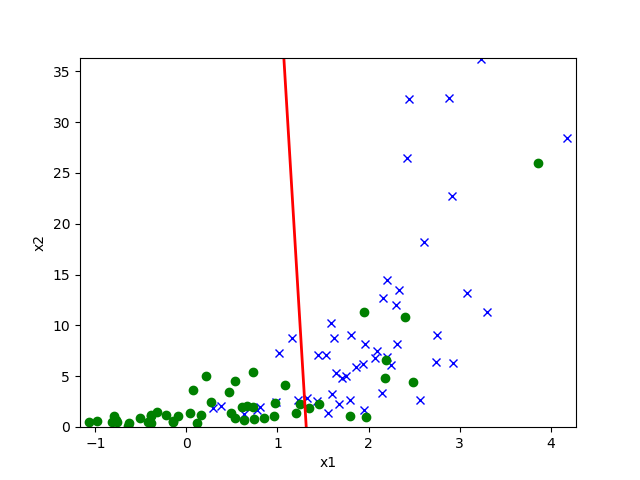
\includegraphics[width=0.65\linewidth]{01-linearclass/p01e_pred_1.png}
    \caption{Separating hyperplane for GDA on the validation set for Dataset 1. Visual impaired students can access the corresponding desmos plot \href{https://www.desmos.com/calculator/sumhryvopb}{here} (Note: This is for reference only.  You are not required to submit a plot.)}
\end{figure}

	\input{01-linearclass/06-plot-ds1}
	\input{01-linearclass/07-plot-ds2}
	\input{01-linearclass/08-transform}
\end{enumerate}

\textbf{Once you are done with src-linear, please copy over your src-linear/submission/logreg.py to src-incomplete and src-imbalanced by running}
\begin{enumerate}
	\item \texttt{cp ./src-linear/submission/logreg.py ./src-incomplete}
	\item \texttt{cp ./src-linear/submission/logreg.py ./src-imbalanced}
\end{enumerate}
